\section{Results}
\label{sec:results}

\subsection{Reproduction}
\label{sec:res-repro}

Before changing anything we reproduced the published method from its released code on its own tasks. On JNU the mean
accuracy over the six condition pairs is \SI{98.03}{\percent} against \SI{98.50}{\percent} reported; on Paderborn it is
\SI{96.20}{\percent} against \SI{96.78}{\percent}. The two hardest tasks bracket the published values over four seeds
(A3$\to$A2: $93.9\pm4.7$ against 97.84 reported; A1$\to$A2: $90.3\pm4.9$ against 87.03), and the seed standard deviation on
those tasks, about 5 points, exceeds many differences reported between competing methods in this literature. We treat the
method as reproduced and use the released hyper-parameters unchanged from here on.

\subsection{What survives bearing-disjoint evaluation}
\label{sec:res-collapse}

\begin{table}[htbp]
\centering
\caption{Paderborn: accuracy (\%) of SDALR (final checkpoint, seed 2024) on leaky and bearing-disjoint (clean) targets, with the envelope threshold gate and the oracle pseudo-label filter. Each entry is the mean over the six condition pairs of that split.}
\label{tab:collapse}
\small
\setlength{\tabcolsep}{4pt}
\begin{tabular}{lrrrrrrr}
\toprule
Split & Leaky & Clean & $\Delta_{\mathrm{leak}}$ & Gated & Gain & Oracle & Recoverable (\%) \\
\midrule
S00 & 91.5 & 66.5 & 25.0 & 69.7 & +3.1 & 89.0 & 90 \\
S01 & 96.1 & 39.8 & 56.3 & 62.5 & +22.6 & 95.1 & 98 \\
S02 & 88.8 & 51.6 & 37.2 & 60.9 & +9.3 & 73.9 & 60 \\
S03 & 93.8 & 58.6 & 35.2 & 57.2 & -1.5 & 75.5 & 48 \\
S04 & 82.2 & 74.0 & 8.2 & 77.6 & +3.6 & 92.1 & 222 \\
S05 & 98.0 & 36.4 & 61.6 & 45.4 & +9.0 & 85.1 & 79 \\
S06 & 90.2 & 68.6 & 21.6 & 73.3 & +4.7 & 83.3 & 68 \\
S07 & 99.2 & 51.5 & 47.8 & 52.1 & +0.7 & 91.9 & 85 \\
S08 & 97.1 & 37.6 & 59.4 & 60.0 & +22.3 & 91.1 & 90 \\
S09 & 89.5 & 60.1 & 29.4 & 64.4 & +4.3 & 82.5 & 76 \\
\midrule
fold A & 88.3 & 58.4 & 30.0 & 61.2 & +4.4 & 88.5 & 101 \\
fold B & 99.9 & 55.3 & 44.6 & 62.3 & +7.0 & 76.8 & 48 \\
\bottomrule
\end{tabular}
\begin{minipage}{\linewidth}\vspace{2pt}\footnotesize Median over the ten random splits: $\Delta_{\mathrm{leak}}$ 36.2~pp (range 8.2--61.6, one-sided Wilcoxon $p=0.001$); gate gain +4.5~pp (positive in 9/10, $p=0.003$); filter-recoverable share 82\,\%. The two mechanical folds are listed below the rule and are not pooled into these statistics; for them the leaky and clean arms come from the fold job, while the gated and oracle arms come from the gating job and their gain and recoverable share are computed against that job's own ungated clean arm (56.8 and 55.3\,\% for folds A and B). Differences are computed before rounding and may differ by 0.1 from the difference of the displayed values.\end{minipage}
\end{table}


\begin{figure}[htbp]
\centering
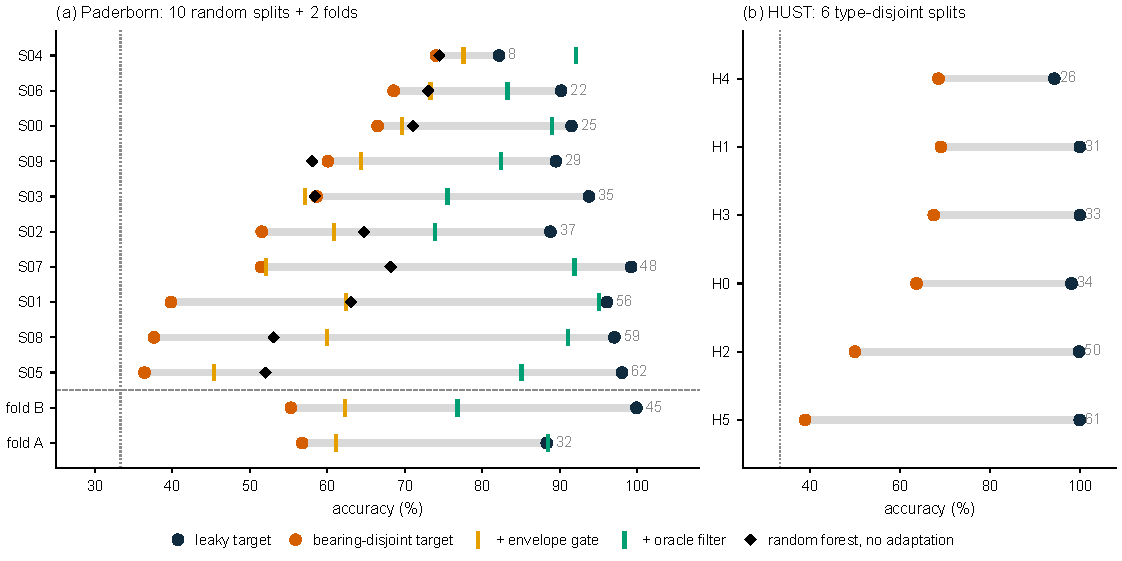
\includegraphics[width=\linewidth]{figures/fig2_collapse.pdf}
\caption{Accuracy by split on both rigs, rows sorted by the size of the collapse. Each row joins the leaky target (dark) to
the bearing-disjoint target (orange); ticks mark the same source model adapted with the envelope threshold gate (amber) and
with the oracle pseudo-label filter (green), and diamonds a random forest on ten time-domain statistics trained on the same
source windows without adaptation. The number at the right of each row is $\Delta_{\mathrm{leak}}$ in percentage points.
(a) Paderborn, ten pre-registered random bearing splits above the rule and the two mechanical folds below it; (b) HUST
bearing, six type-disjoint splits. Dotted line: three-class chance level.}
\label{fig:collapse}
\end{figure}

On the two mechanical folds, SDALR reaches \SI{94.1}{\percent} on leaky targets and \SI{56.8}{\percent} on bearing-disjoint
targets, both arms from the same job: a loss of 30.0 points with fold~A as source and 44.6 points with fold~B, 37.3 points
pooled over the 12 paired tasks. The task-level test reaches the smallest attainable value ($p=0.00024$) but treats tasks
that share source checkpoints as independent; the honest cluster-level test on two folds cannot fall below $p=0.25$, so
these two folds are descriptive and the ten random splits below carry the inference. The released checkpoint policy, which
consults target labels, gives \SI{94.7}{\percent} against \SI{57.8}{\percent}: target-label selection is worth 0.0--2.0
points and adaptation itself 2.2--5.4 points on clean targets, so neither accounts for the gap.
With fold B as source, all six leaky tasks exceed \SI{99.7}{\percent} while all six clean tasks fall between \SI{55.27}{}
and \SI{55.33}{\percent}.

Across the ten pre-registered random splits (Table~\ref{tab:collapse}, Fig.~\ref{fig:collapse}) the split-level loss has a
median of 36.2 points with a range of 8.2--61.6, which survives a cluster-level permutation test and Benjamini--Hochberg
adjustment ($p=0.001$, $p_{\mathrm{BH}}=0.005$), so the effect is not an artefact of the two mechanical folds.
The spread across splits is itself informative: which bearings happen to be in the source set moves clean accuracy between
\SI{36.4}{} and \SI{74.0}{\percent}, which is why a single split --- the norm in this literature --- cannot support a
performance claim.

\subsection{The collapse is not specific to one method}
\label{sec:res-second}

\begin{table}[htbp]
\centering
\caption{The collapse is not specific to one method: two source-free methods and four non-adaptive random forests on Paderborn, leaky versus bearing-disjoint targets (accuracy, \%).}
\label{tab:methods}
\begin{tabular}{lrrrr}
\toprule
Method & Leaky & Clean & $\Delta_{\mathrm{leak}}$ & $p$ \\
\midrule
SDALR, as released (target-label checkpoint) & 94.7 & 57.8 & 36.9 & 0.0002 \\
SDALR, final checkpoint & 94.1 & 56.8 & 37.3 & 0.0002 \\
SHOT, final iterate & 87.2 & 65.1 & 22.1 & 0.0012 \\
\midrule
Random forest, 10 time statistics & 88.8 & 63.6 & 25.2 & 0.0017 \\
Random forest, 64 spectral bands & 93.2 & 52.6 & 40.6 & 0.0002 \\
Random forest, envelope spectrum & 76.7 & 43.1 & 33.5 & 0.0002 \\
Random forest, all three feature sets & 95.4 & 60.3 & 35.1 & 0.0002 \\
\bottomrule
\end{tabular}
\begin{minipage}{\linewidth}\vspace{2pt}\footnotesize All rows use the same windows, the same two mechanical folds and the same 12 paired tasks; the random forests use no adaptation and no target data. $p$ is a one-sided Wilcoxon signed-rank test over those tasks, for which the smallest attainable value is $2^{-12}=0.00024$. Tasks within a fold share source checkpoints, so these $p$-values are descriptive; cluster-level tests are reported in Section~\ref{sec:protocol}. Differences are computed before rounding.\end{minipage}
\end{table}


\begin{table}[htbp]
\centering
\caption{Second rig: SDALR on HUST bearing, six pre-registered type-disjoint splits (accuracy, \%). The source is three bearing types; the clean target is the other two at the target load.}
\label{tab:hust}
\begin{tabular}{llrrr}
\toprule
Split & Source bearings & Leaky & Clean & $\Delta_{\mathrm{leak}}$ \\
\midrule
H0 & 6204, 6207, 6208 & 98.1 & 63.7 & 34.5 \\
H1 & 6204, 6205, 6207 & 100.0 & 69.1 & 30.9 \\
H2 & 6204, 6205, 6206 & 99.8 & 49.9 & 49.9 \\
H3 & 6205, 6206, 6207 & 100.0 & 67.5 & 32.5 \\
H4 & 6206, 6207, 6208 & 94.3 & 68.5 & 25.8 \\
H5 & 6205, 6206, 6208 & 100.0 & 38.9 & 61.1 \\
\bottomrule
\end{tabular}
\begin{minipage}{\linewidth}\vspace{2pt}\footnotesize Median $\Delta_{\mathrm{leak}}$ 33.5~pp (range 25.8--61.1, one-sided Wilcoxon $p=0.016$), which meets the replication rule fixed before the run. On this rig the clean target changes bearing size as well as bearing identity, so the shift is stronger than Paderborn's.\end{minipage}
\end{table}


Table~\ref{tab:methods} repeats the paired design for a second source-free method and for non-adaptive baselines. SHOT falls
from \SI{87.2}{} to \SI{65.1}{\percent} ($-22.1$ points, $p=0.001$). Random forests \cite{pedregosa2011sklearn} trained on the same source windows
with no adaptation at all collapse in the same way, by 25.2 points on ten time-domain statistics and by 40.7 and 33.5 points on
spectral-band and envelope-spectrum features. Bearing-disjoint evaluation therefore does not expose a weakness of one
adaptation algorithm; it exposes a property of models trained on a handful of physical bearings.

The result also replicates on a second rig. On HUST bearing (Table~\ref{tab:hust}, Fig.~\ref{fig:collapse}(b)) mean leaky accuracy
is \SI{98.7}{\percent} --- the near-ceiling figure this literature usually reports --- and mean clean accuracy is
\SI{59.6}{\percent}, with a median split-level loss of 33.5 points ($p=0.016$), meeting the replication rule fixed before
the run. On this rig the disjoint target changes bearing size as well as bearing identity, so the shift is stronger than
Paderborn's and the result is stated as identity \emph{and} geometry.

\subsection{What the adapted model does instead}
\label{sec:res-mechanism}

\begin{figure}[htbp]
\centering
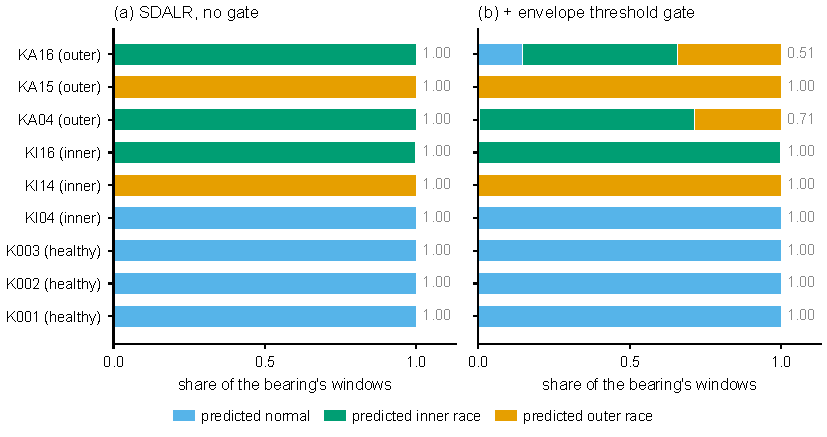
\includegraphics[width=\linewidth]{figures/fig3_purity.pdf}
\caption{Per-bearing label purity on bearing-disjoint targets: the share of a physical bearing's windows receiving that
bearing's most frequent predicted label, with the predicted label annotated. Purity 1.0 means the model gave one label to
the entire specimen.}
\label{fig:purity}
\end{figure}

Saved per-window predictions explain the numbers above. Purity is measured over all six tasks of a direction: the share of a
bearing's windows that receive its most frequent predicted label. On the bearing-disjoint targets of the fold~B direction it
is 1.000 for every bearing (Fig.~\ref{fig:purity}a). Healthy bearings are labelled healthy; among faulty bearings, KA04 and
KA16 are labelled inner race, KI04 normal and KI14 outer race. The resulting accuracy of \SI{55.3}{\percent} is arithmetic
rather than noise: with three bearings per class each labelled as a block, the three healthy bearings are right and one of
three bearings in each fault class is right, giving $5/9 = \SI{55.6}{\percent}$ up to the small imbalance in windows per
bearing. The adapted model is not making noisy per-window decisions on unseen specimens --- it is assigning one
identity-level label to each specimen.

\subsection{How much any pseudo-label filter could repair}
\label{sec:res-decomp}

\begin{figure}[htbp]
\centering
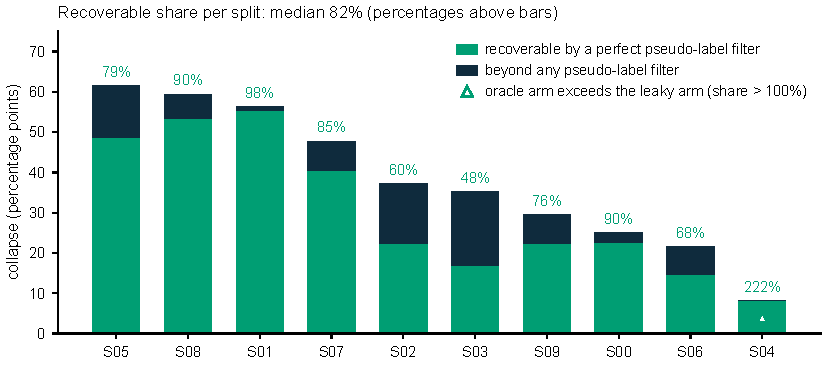
\includegraphics[width=\linewidth]{figures/fig4_decomposition.pdf}
\caption{Decomposition~\eqref{eq:decomp} per split: the part of the collapse an oracle pseudo-label filter recovers, and the
part that remains when every kept pseudo-label is correct.}
\label{fig:decomp}
\end{figure}

We apply~\eqref{eq:decomp} to the ten random splits, where all four arms of a split are produced in one job and are
therefore directly comparable. The filter-recoverable share has a median of \SI{82}{\percent} (interquartile range
68--\SI{90}{\percent}, Fig.~\ref{fig:decomp}) and varies strongly: at \SI{48}{\percent} on S03 half the collapse lies in the
source representation, while on S04 --- the mildest collapse, 8.2 points --- the oracle arm exceeds even the leaky arm, so
its share of \SI{222}{\percent} carries no upper-bound reading. The two mechanical folds behave the same way (fold~A
\SI{106}{\percent}, fold~B \SI{48}{\percent}).

The quantity being bounded should be stated precisely. The oracle arm withholds every incorrect pseudo-label and keeps every
correct one, so it bounds \emph{keep-or-withhold filters acting on this method's pseudo-label step} --- the family to which
all four gates belong. It does not bound methods that relabel samples, reweight them continuously, or change the
representation; and where it exceeds the leaky arm it is not a bound at all, but evidence that a cleaner pseudo-label set can
beat same-bearing training. With that reading, a perfect pseudo-label filter still leaves a median of about one-fifth of the
collapse untouched on this rig, and half of it on some splits.

\subsection{Physics gating: safety, paired gains and the ceiling}
\label{sec:res-gating}

\begin{table}[htbp]
\centering
\caption{Gate safety on real healthy bearings. A false acceptance is a healthy recording given a fault verdict.}
\label{tab:gates}
\small
\setlength{\tabcolsep}{4pt}
\begin{tabular}{lrrrr}
\toprule
Gate (swept parameter) & Operating point & Healthy false acceptance & Correct verdicts & At zero FA \\
\midrule
Envelope threshold rule (PCV-style), $z$ & 10 & 1/480 & 366 & 351 \\
Shaft-alias-guarded comb (comb\_v2), $\alpha$ & 0.05 & 0/480 & 312 & 312 \\
Surrogate-null comb test, $\alpha$ & 0.05 & 9/480 & 309 & -- \\
Raw-spectrum band rule (EAGLE-style), $z$ & 2 & 214/480 & 429 & 0 \\
\bottomrule
\end{tabular}
\begin{minipage}{\linewidth}\vspace{2pt}\footnotesize Population: 2{,}319 Paderborn recordings (480 healthy, 1{,}839 single inner- or outer-race). Operating points are the values fixed before the gates were evaluated. The last column sweeps each gate's parameter and reports the largest number of correct fault verdicts reachable while accepting no healthy recording. Full operating curves: Supplementary~S2. The population spans 29 physical bearings -- 6 healthy, 11 real-damage and 12 artificial-damage -- at all four operating conditions; coverage by damage origin is given in Section~\ref{sec:res-gating}.\end{minipage}
\end{table}


\begin{figure}[htbp]
\centering
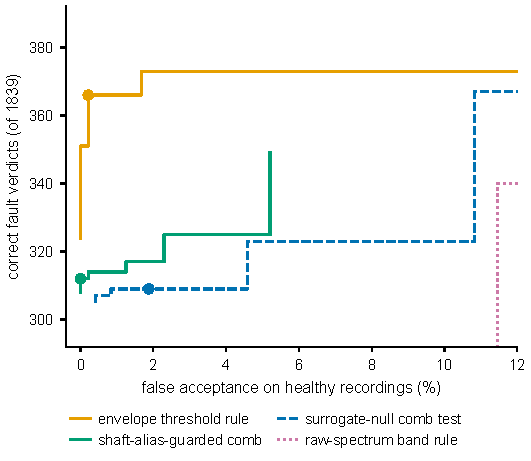
\includegraphics[width=0.8\linewidth]{figures/fig5_roc.pdf}
\caption{Gate operating curves on 2319 Paderborn recordings: correct fault verdicts against false acceptance on the 480
healthy recordings, as each gate's parameter is swept. Filled circles mark the operating points fixed before evaluation. The
envelope threshold rule lies on or above the others everywhere. The vertical range starts at 292 verdicts: the raw-spectrum
band rule returns no correct verdict below \SI{10.8}{\percent} false acceptance, and its own operating point lies at
\SI{45}{\percent}, off the right of the axis.}
\label{fig:roc}
\end{figure}

\textbf{The population.} Gate behaviour is characterised on all 2319 single-fault and healthy Paderborn recordings, spanning
29 physical bearings at all four operating conditions: 6 healthy, 11 real-damage and 12 artificial-damage (electro-discharge
machining, drilling, manual indentation). The adaptation experiments use only the healthy and real-damage bearings at three
of those conditions, so coverage is read separately by damage origin: at the pre-registered operating point the envelope
threshold rule engages 7 of the 11 real-damage bearings (209 of their 880 recordings) and 6 of the 12 artificial ones, the
alias-guarded comb 5 of 11, and the raw-spectrum rule 9 of 11 while accepting \SI{45}{\percent} of healthy recordings. Only
the real-damage figures bear on the gating results inside adaptation.

At the operating points fixed before evaluation (Table~\ref{tab:gates}), the envelope threshold rule accepts a fault label
on 1 of 480 healthy recordings, the shaft-alias-guarded comb on none, the surrogate-null comb on 9, and the raw-spectrum
band rule on 214 --- \SI{45}{\percent} of healthy machinery declared faulty. Sweeping each gate's parameter
(Fig.~\ref{fig:roc}) confirms this is not a threshold artefact: the envelope rule dominates at every false-acceptance level,
the alias guard improves the comb test, and the raw-spectrum rule is dominated everywhere. Coverage is the binding
constraint for all of them: no gate exceeds \SI{24}{\percent} correct fault verdicts before false acceptance passes
\SI{10}{\percent}, and the envelope gates engage 7 of the 11 real-damage bearings, on about a quarter of their recordings.
The operating points were fixed in the protocol before any gate was evaluated; the sweep is reported as a sensitivity
analysis, not as a selection step. Gate verdicts themselves use no target labels, but we note that an operating point
transferred to a new rig would need its own healthy recordings to be characterised, which is a deployment requirement rather
than a source-free violation.

\begin{table}[htbp]
\centering
\caption{Paired per-task effect of gating inside SDALR on the 12 bearing-disjoint tasks of the two mechanical folds (gated $-$ ungated, percentage points).}
\label{tab:gains}
\small
\setlength{\tabcolsep}{4pt}
\begin{tabular}{llrrrrrr}
\toprule
Gate & Seed & Mean & Median & Min & Max & Tasks $>0$ & $p$ \\
\midrule
Shaft-alias-guarded comb & 0 & +3.79 & +3.33 & -0.08 & +11.01 & 7/12 & 0.0078 \\
 & 1 & +4.56 & +3.28 & -0.08 & +15.45 & 8/12 & 0.0068 \\
 & 2024 & +3.73 & +3.67 & -0.05 & +8.07 & 8/12 & 0.0068 \\
\midrule
Envelope threshold rule & 0 & +7.44 & +7.57 & -0.01 & +18.02 & 9/12 & 0.0020 \\
 & 1 & +7.99 & +6.65 & -0.70 & +19.44 & 10/12 & 0.0017 \\
 & 2024 & +5.70 & +5.59 & -0.05 & +14.52 & 10/12 & 0.0010 \\
\bottomrule
\end{tabular}
\begin{minipage}{\linewidth}\vspace{2pt}\footnotesize Every arm of a comparison runs in one job on the same source checkpoint, verified from identical pre-update target accuracy in each adaptation log, so these are paired differences. The between-seed spread of the per-task gain is 1.7~pp (comb) and 2.4~pp (envelope), against 2.8~pp for ungated per-task accuracy.\end{minipage}
\end{table}


\begin{figure}[htbp]
\centering
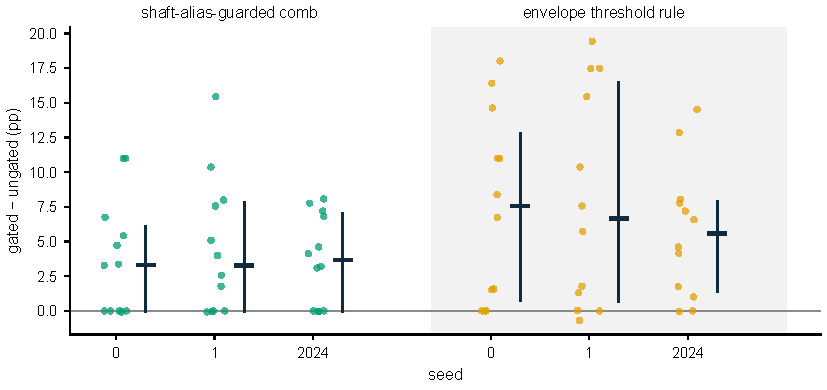
\includegraphics[width=\linewidth]{figures/fig6_gains.pdf}
\caption{Paired per-task effect of inserting each gate into the adaptation loop, over three seeds. Each point is one task;
positive values are gains over the ungated arm trained from the same source checkpoint.}
\label{fig:gains}
\end{figure}

Inside the adaptation loop the two safe gates help, consistently and modestly (Table~\ref{tab:gains},
Fig.~\ref{fig:gains}). Over three seeds the mean paired gain is $+4.03$ points for the alias-guarded comb ($p=0.007$) and
$+7.05$ points for the envelope threshold rule ($p=0.0007$), positive in every seed, and no gated task loses more than 0.70
points. The paired design matters here: the between-seed spread of the per-task gain is 1.7 and 2.4 points, against 2.8
points for ungated per-task accuracy, so an unpaired comparison of means at this scale would be uninformative. Over the ten
random splits the median gain is $+4.5$ points, positive in 9 of 10 ($p=0.003$). The unsafe raw-spectrum rule lowers
accuracy by 3.9 points, as its false-acceptance rate predicts.

Measured against the ceiling of Section~\ref{sec:res-decomp}, the envelope gate closes a median of \SI{19}{\percent} of the
oracle gap. Where it engages a bearing it does break the identity lock --- on the bearing KA04 the label purity falls from
1.00 to 0.56 and one task rises from \SI{55.3}{} to \SI{69.9}{\percent} --- but it cannot act on the bearings it never
engages, nor on the part of the collapse that no filter can reach. The modest size of the gain is therefore a property of
the problem, not of the tuning.

\subsection{Bearing identity in the source representation}
\label{sec:res-probe}

The decomposition says part of the damage is in the representation; a probe shows what is in it. On the frozen source
features we fit a logistic-regression probe with record-disjoint halves, one probe per class, each required to tell apart
the bearings \emph{within} that class --- a task that carries no class information at all. Pooled over the six source models
(two folds $\times$ three source conditions), the probe identifies the correct physical bearing in 507 of 508 held-out
recordings, against a pooled chance level of 0.35. Those 508 recordings are the ones falling in the held-out half of the
deterministic hash split, which divides the 1080 source recordings 508/572 rather than exactly in half. Individual specimens
are therefore almost perfectly encoded before adaptation begins.

Identity is not something the network invents. The identical probe on ten elementary time-domain statistics of the same
windows identifies the bearing in 508 of 508 recordings ($p < 10^{-200}$ against the same chance level): the shortcut is
already present in the raw signals. That is why non-adaptive random forests collapse in the same way, and why an adaptation
objective has no reason to prefer fault physics over specimen identity --- on a rig with three bearings per class, identity
separates the source classes as effectively as the fault signature does, at no cost to the source loss. One caveat applies
to both probes: the source model was trained on other windows of the same recordings, so they measure what the
representation encodes about bearings the model has seen, not generalisation to new specimens.

\subsection{Cage slip and the shaft-order lock of 6203 bearings}
\label{sec:res-slip}

\begin{figure}[htbp]
\centering
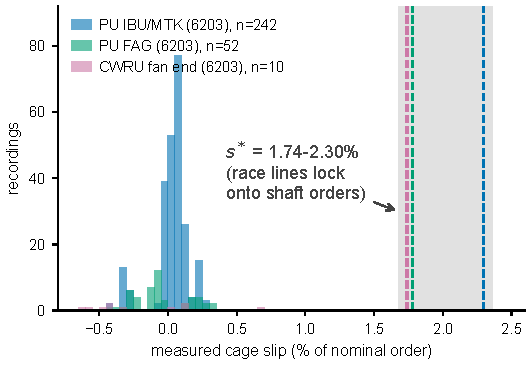
\includegraphics[width=0.85\linewidth]{figures/fig7_slip.pdf}
\caption{Measured cage slip from fault lines with per-recording measured speed. The dashed lines mark $s^\ast$, the slip at
which the outer- and inner-race lines of each 6203 geometry reach integer shaft orders simultaneously.}
\label{fig:slip}
\end{figure}

A kinematic remark closes the results, because it bears on every gate that places windows by geometry. Under the cage-slip
model $\mathrm{BPFO}(s)=(1-s)\,\mathrm{BPFO}_0$ and $\mathrm{BPFO}(s)+\mathrm{BPFI}(s)=n$, so if
$\mathrm{BPFO}_0=m+\delta$ with $m$ integer, both race lines reach integer shaft orders at the same slip
$s^\ast=\delta/\mathrm{BPFO}_0$: \SI{2.30}{\percent} for the Paderborn IBU/MTK geometry, \SI{1.78}{\percent} for the FAG
geometry and \SI{1.74}{\percent} for the CWRU fan-end bearing. Smith and Randall observed such lock-like behaviour on the CWRU fan-end bearing and
noted that it makes a definite diagnosis difficult \cite{smith2015}; the contrary view, that such lines can always be
separated given sufficient spectral resolution, appears for instance in the patent literature \cite{patent10168248}.

We tested whether it occurs in practice by measuring slip directly. Fault-line positions were fitted against the measured
shaft speed on every recording with at least two lit harmonics; on synthetic signals with injected slips of \SI{0.1}{} to
\SI{4}{\percent} the estimator recovers the truth to within \SI{0.17}{\percent}. Measured slip on Paderborn has a median of
\SI{0.06}{\percent} with a 5--95\% range of $-0.31$ to $+\SI{0.22}{\percent}$ (Fig.~\ref{fig:slip}), an order of magnitude
below $s^\ast$. Of 304 measurable 6203 recordings, three fall within tolerance of $s^\ast$, and all three fail once
shaft-order bins are masked, which identifies them as shaft pickup rather than fault lines. By the criterion fixed before
the measurement, the lock is therefore a curiosity on these rigs rather than a practical failure mode, and we report it as
such; the textbook slip range of 1--\SI{2}{\percent} does not describe these operating points. The residual offset of about
$-\SI{0.3}{\percent}$ on CWRU, where speed is logged rather than measured, bounds how precisely any fixed-kinematics window
can be placed.
